% Graphic for TeX using PGF
% Title: /home/maximilien/INSA/alambic/report/draw/multiple_doc_completion.dia
% Creator: Dia v0.97.3
% CreationDate: Wed Apr 29 09:27:53 2015
% For: maximilien
% \usepackage{tikz}
% The following commands are not supported in PSTricks at present
% We define them conditionally, so when they are implemented,
% this pgf file will use them.
\ifx\du\undefined
  \newlength{\du}
\fi
\setlength{\du}{15\unitlength}
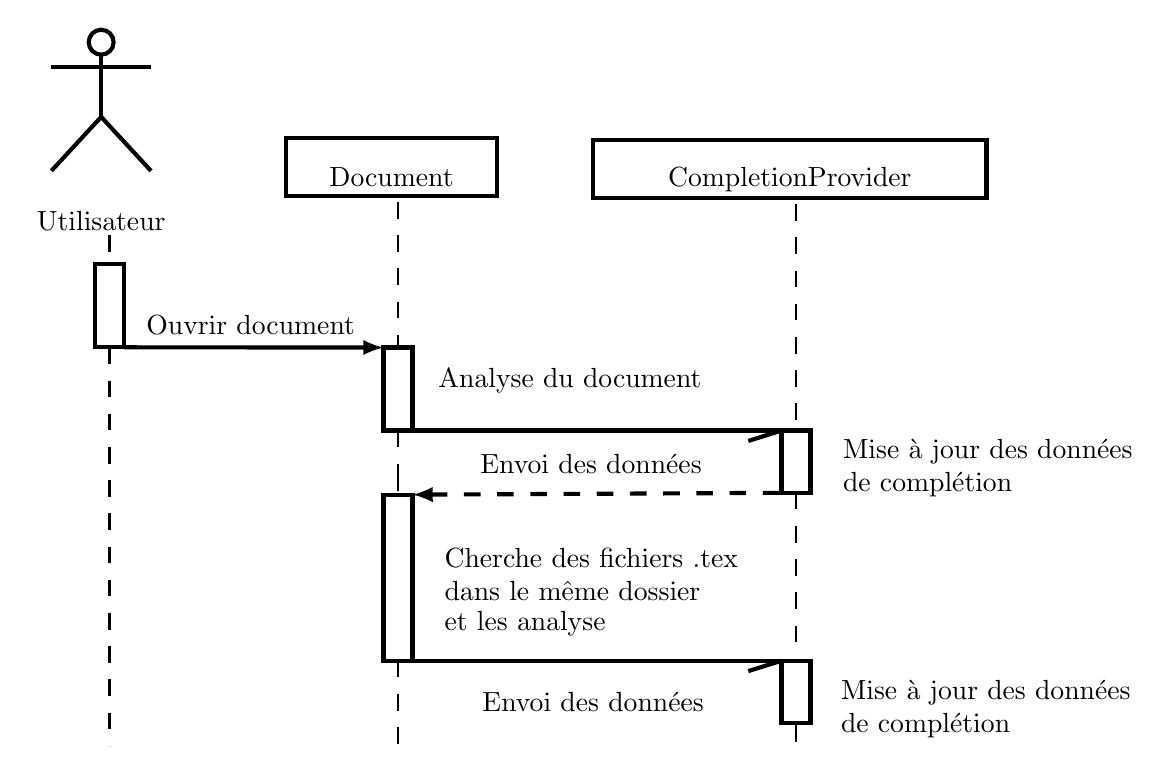
\begin{tikzpicture}
\pgftransformxscale{1.000000}
\pgftransformyscale{-1.000000}
\definecolor{dialinecolor}{rgb}{0.000000, 0.000000, 0.000000}
\pgfsetstrokecolor{dialinecolor}
\definecolor{dialinecolor}{rgb}{1.000000, 1.000000, 1.000000}
\pgfsetfillcolor{dialinecolor}
\pgfsetlinewidth{0.100000\du}
\pgfsetdash{}{0pt}
\definecolor{dialinecolor}{rgb}{1.000000, 1.000000, 1.000000}
\pgfsetfillcolor{dialinecolor}
\pgfpathellipse{\pgfpoint{-28.150000\du}{2.050000\du}}{\pgfpoint{0.300000\du}{0\du}}{\pgfpoint{0\du}{0.300000\du}}
\pgfusepath{fill}
\definecolor{dialinecolor}{rgb}{0.000000, 0.000000, 0.000000}
\pgfsetstrokecolor{dialinecolor}
\pgfpathellipse{\pgfpoint{-28.150000\du}{2.050000\du}}{\pgfpoint{0.300000\du}{0\du}}{\pgfpoint{0\du}{0.300000\du}}
\pgfusepath{stroke}
\definecolor{dialinecolor}{rgb}{0.000000, 0.000000, 0.000000}
\pgfsetstrokecolor{dialinecolor}
\draw (-29.350000\du,2.650000\du)--(-26.950000\du,2.650000\du);
\definecolor{dialinecolor}{rgb}{0.000000, 0.000000, 0.000000}
\pgfsetstrokecolor{dialinecolor}
\draw (-28.150000\du,2.350000\du)--(-28.150000\du,3.850000\du);
\definecolor{dialinecolor}{rgb}{0.000000, 0.000000, 0.000000}
\pgfsetstrokecolor{dialinecolor}
\draw (-28.150000\du,3.850000\du)--(-29.350000\du,5.150000\du);
\definecolor{dialinecolor}{rgb}{0.000000, 0.000000, 0.000000}
\pgfsetstrokecolor{dialinecolor}
\draw (-28.150000\du,3.850000\du)--(-26.950000\du,5.150000\du);
% setfont left to latex
\definecolor{dialinecolor}{rgb}{0.000000, 0.000000, 0.000000}
\pgfsetstrokecolor{dialinecolor}
\node at (-28.150000\du,6.345000\du){Utilisateur};
\pgfsetlinewidth{0.100000\du}
\pgfsetdash{}{0pt}
\definecolor{dialinecolor}{rgb}{1.000000, 1.000000, 1.000000}
\pgfsetfillcolor{dialinecolor}
\fill (-16.300000\du,4.400000\du)--(-16.300000\du,5.800000\du)--(-6.822500\du,5.800000\du)--(-6.822500\du,4.400000\du)--cycle;
\definecolor{dialinecolor}{rgb}{0.000000, 0.000000, 0.000000}
\pgfsetstrokecolor{dialinecolor}
\draw (-16.300000\du,4.400000\du)--(-16.300000\du,5.800000\du)--(-6.822500\du,5.800000\du)--(-6.822500\du,4.400000\du)--cycle;
% setfont left to latex
\definecolor{dialinecolor}{rgb}{0.000000, 0.000000, 0.000000}
\pgfsetstrokecolor{dialinecolor}
\node at (-11.561250\du,5.350000\du){CompletionProvider};
\pgfsetlinewidth{0.050000\du}
\pgfsetdash{}{0pt}
\pgfsetdash{{0.400000\du}{0.400000\du}}{0\du}
\definecolor{dialinecolor}{rgb}{0.000000, 0.000000, 0.000000}
\pgfsetstrokecolor{dialinecolor}
\draw (-27.950000\du,6.700000\du)--(-27.950000\du,7.400000\du);
\definecolor{dialinecolor}{rgb}{0.000000, 0.000000, 0.000000}
\pgfsetstrokecolor{dialinecolor}
\draw (-27.950000\du,9.400000\du)--(-27.950000\du,19.000000\du);
\pgfsetlinewidth{0.100000\du}
\pgfsetdash{}{0pt}
\definecolor{dialinecolor}{rgb}{1.000000, 1.000000, 1.000000}
\pgfsetfillcolor{dialinecolor}
\fill (-28.300000\du,7.400000\du)--(-28.300000\du,9.400000\du)--(-27.600000\du,9.400000\du)--(-27.600000\du,7.400000\du)--cycle;
\definecolor{dialinecolor}{rgb}{0.000000, 0.000000, 0.000000}
\pgfsetstrokecolor{dialinecolor}
\draw (-28.300000\du,7.400000\du)--(-28.300000\du,9.400000\du)--(-27.600000\du,9.400000\du)--(-27.600000\du,7.400000\du)--cycle;
\pgfsetlinewidth{0.100000\du}
\pgfsetdash{}{0pt}
\definecolor{dialinecolor}{rgb}{1.000000, 1.000000, 1.000000}
\pgfsetfillcolor{dialinecolor}
\fill (-23.700000\du,4.350000\du)--(-23.700000\du,5.750000\du)--(-18.612500\du,5.750000\du)--(-18.612500\du,4.350000\du)--cycle;
\definecolor{dialinecolor}{rgb}{0.000000, 0.000000, 0.000000}
\pgfsetstrokecolor{dialinecolor}
\draw (-23.700000\du,4.350000\du)--(-23.700000\du,5.750000\du)--(-18.612500\du,5.750000\du)--(-18.612500\du,4.350000\du)--cycle;
% setfont left to latex
\definecolor{dialinecolor}{rgb}{0.000000, 0.000000, 0.000000}
\pgfsetstrokecolor{dialinecolor}
\node at (-21.156250\du,5.300000\du){Document};
\pgfsetlinewidth{0.050000\du}
\pgfsetdash{}{0pt}
\pgfsetdash{{0.400000\du}{0.400000\du}}{0\du}
\definecolor{dialinecolor}{rgb}{0.000000, 0.000000, 0.000000}
\pgfsetstrokecolor{dialinecolor}
\draw (-21.000000\du,5.900000\du)--(-21.000000\du,9.405599\du);
\definecolor{dialinecolor}{rgb}{0.000000, 0.000000, 0.000000}
\pgfsetstrokecolor{dialinecolor}
\draw (-21.000000\du,11.405599\du)--(-21.000000\du,13.450000\du);
\pgfsetlinewidth{0.100000\du}
\pgfsetdash{}{0pt}
\definecolor{dialinecolor}{rgb}{1.000000, 1.000000, 1.000000}
\pgfsetfillcolor{dialinecolor}
\fill (-21.350000\du,9.405599\du)--(-21.350000\du,11.405599\du)--(-20.650000\du,11.405599\du)--(-20.650000\du,9.405599\du)--cycle;
\definecolor{dialinecolor}{rgb}{0.000000, 0.000000, 0.000000}
\pgfsetstrokecolor{dialinecolor}
\draw (-21.350000\du,9.405599\du)--(-21.350000\du,11.405599\du)--(-20.650000\du,11.405599\du)--(-20.650000\du,9.405599\du)--cycle;
\pgfsetlinewidth{0.050000\du}
\pgfsetdash{}{0pt}
\pgfsetdash{{0.400000\du}{0.400000\du}}{0\du}
\definecolor{dialinecolor}{rgb}{0.000000, 0.000000, 0.000000}
\pgfsetstrokecolor{dialinecolor}
\draw (-11.411300\du,5.950000\du)--(-11.411300\du,11.405599\du);
\definecolor{dialinecolor}{rgb}{0.000000, 0.000000, 0.000000}
\pgfsetstrokecolor{dialinecolor}
\draw (-11.411300\du,12.905599\du)--(-11.411300\du,19.000000\du);
\pgfsetlinewidth{0.100000\du}
\pgfsetdash{}{0pt}
\definecolor{dialinecolor}{rgb}{1.000000, 1.000000, 1.000000}
\pgfsetfillcolor{dialinecolor}
\fill (-11.761300\du,11.405599\du)--(-11.761300\du,12.905599\du)--(-11.061300\du,12.905599\du)--(-11.061300\du,11.405599\du)--cycle;
\definecolor{dialinecolor}{rgb}{0.000000, 0.000000, 0.000000}
\pgfsetstrokecolor{dialinecolor}
\draw (-11.761300\du,11.405599\du)--(-11.761300\du,12.905599\du)--(-11.061300\du,12.905599\du)--(-11.061300\du,11.405599\du)--cycle;
\pgfsetlinewidth{0.100000\du}
\pgfsetbuttcap
\pgfsetdash{}{0pt}
{
\definecolor{dialinecolor}{rgb}{0.000000, 0.000000, 0.000000}
\pgfsetfillcolor{dialinecolor}
% was here!!!
\pgfsetarrowsstart{latex}
\definecolor{dialinecolor}{rgb}{0.000000, 0.000000, 0.000000}
\pgfsetstrokecolor{dialinecolor}
\draw (-21.350000\du,9.405600\du)--(-27.600000\du,9.400000\du);
}
% setfont left to latex
\definecolor{dialinecolor}{rgb}{0.000000, 0.000000, 0.000000}
\pgfsetstrokecolor{dialinecolor}
\node at (-24.550000\du,8.852800\du){Ouvrir document};
% setfont left to latex
\definecolor{dialinecolor}{rgb}{0.000000, 0.000000, 0.000000}
\pgfsetstrokecolor{dialinecolor}
\node[anchor=west] at (-20.300000\du,10.200000\du){Analyse du document};
\pgfsetlinewidth{0.100000\du}
\pgfsetbuttcap
\pgfsetdash{}{0pt}
{
\definecolor{dialinecolor}{rgb}{0.000000, 0.000000, 0.000000}
\pgfsetfillcolor{dialinecolor}
% was here!!!
\definecolor{dialinecolor}{rgb}{0.000000, 0.000000, 0.000000}
\pgfsetstrokecolor{dialinecolor}
\draw (-11.761300\du,11.405599\du)--(-20.650000\du,11.405600\du);
}
\definecolor{dialinecolor}{rgb}{0.000000, 0.000000, 0.000000}
\pgfsetstrokecolor{dialinecolor}
\draw (-11.761300\du,11.405599\du)--(-20.650000\du,11.405600\du);
\pgfsetlinewidth{0.100000\du}
\pgfsetdash{}{0pt}
\pgfsetmiterjoin
\pgfsetbuttcap
\definecolor{dialinecolor}{rgb}{0.000000, 0.000000, 0.000000}
\pgfsetstrokecolor{dialinecolor}
\draw (-12.561300\du,11.655599\du)--(-11.761300\du,11.405599\du)--(-11.761300\du,11.405599\du);
% setfont left to latex
\definecolor{dialinecolor}{rgb}{0.000000, 0.000000, 0.000000}
\pgfsetstrokecolor{dialinecolor}
\node at (-16.350000\du,12.205600\du){Envoi des données};
% setfont left to latex
\definecolor{dialinecolor}{rgb}{0.000000, 0.000000, 0.000000}
\pgfsetstrokecolor{dialinecolor}
\node[anchor=west] at (-10.550000\du,11.900000\du){Mise à jour des données};
% setfont left to latex
\definecolor{dialinecolor}{rgb}{0.000000, 0.000000, 0.000000}
\pgfsetstrokecolor{dialinecolor}
\node[anchor=west] at (-10.550000\du,12.700000\du){de complétion};
\pgfsetlinewidth{0.050000\du}
\pgfsetdash{}{0pt}
\pgfsetdash{{0.400000\du}{0.400000\du}}{0\du}
\definecolor{dialinecolor}{rgb}{0.000000, 0.000000, 0.000000}
\pgfsetstrokecolor{dialinecolor}
\draw (-21.000000\du,12.450000\du)--(-21.000000\du,12.950000\du);
\definecolor{dialinecolor}{rgb}{0.000000, 0.000000, 0.000000}
\pgfsetstrokecolor{dialinecolor}
\draw (-21.000000\du,16.950000\du)--(-21.000000\du,18.950000\du);
\pgfsetlinewidth{0.100000\du}
\pgfsetdash{}{0pt}
\definecolor{dialinecolor}{rgb}{1.000000, 1.000000, 1.000000}
\pgfsetfillcolor{dialinecolor}
\fill (-21.350000\du,12.950000\du)--(-21.350000\du,16.950000\du)--(-20.650000\du,16.950000\du)--(-20.650000\du,12.950000\du)--cycle;
\definecolor{dialinecolor}{rgb}{0.000000, 0.000000, 0.000000}
\pgfsetstrokecolor{dialinecolor}
\draw (-21.350000\du,12.950000\du)--(-21.350000\du,16.950000\du)--(-20.650000\du,16.950000\du)--(-20.650000\du,12.950000\du)--cycle;
\pgfsetlinewidth{0.100000\du}
\pgfsetbuttcap
\pgfsetdash{}{0pt}
\pgfsetdash{{0.400000\du}{0.400000\du}}{0\du}
{
\definecolor{dialinecolor}{rgb}{0.000000, 0.000000, 0.000000}
\pgfsetfillcolor{dialinecolor}
% was here!!!
\pgfsetarrowsstart{latex}
\definecolor{dialinecolor}{rgb}{0.000000, 0.000000, 0.000000}
\pgfsetstrokecolor{dialinecolor}
\draw (-20.650000\du,12.950000\du)--(-11.761300\du,12.905599\du);
}
% setfont left to latex
% setfont left to latex
\definecolor{dialinecolor}{rgb}{0.000000, 0.000000, 0.000000}
\pgfsetstrokecolor{dialinecolor}
\node[anchor=west] at (-10.600000\du,17.715600\du){Mise à jour des données};
% setfont left to latex
\definecolor{dialinecolor}{rgb}{0.000000, 0.000000, 0.000000}
\pgfsetstrokecolor{dialinecolor}
\node[anchor=west] at (-10.600000\du,18.515600\du){de complétion};
\pgfsetlinewidth{0.050000\du}
\pgfsetdash{{0.400000\du}{0.400000\du}}{0\du}
\pgfsetdash{{0.400000\du}{0.400000\du}}{0\du}
\definecolor{dialinecolor}{rgb}{0.000000, 0.000000, 0.000000}
\pgfsetstrokecolor{dialinecolor}
\draw (-11.411300\du,12.905599\du)--(-11.411300\du,16.950000\du);
\definecolor{dialinecolor}{rgb}{0.000000, 0.000000, 0.000000}
\pgfsetstrokecolor{dialinecolor}
\draw (-11.411300\du,18.450000\du)--(-11.411300\du,19.055599\du);
\pgfsetlinewidth{0.100000\du}
\pgfsetdash{}{0pt}
\definecolor{dialinecolor}{rgb}{1.000000, 1.000000, 1.000000}
\pgfsetfillcolor{dialinecolor}
\fill (-11.761300\du,16.950000\du)--(-11.761300\du,18.450000\du)--(-11.061300\du,18.450000\du)--(-11.061300\du,16.950000\du)--cycle;
\definecolor{dialinecolor}{rgb}{0.000000, 0.000000, 0.000000}
\pgfsetstrokecolor{dialinecolor}
\draw (-11.761300\du,16.950000\du)--(-11.761300\du,18.450000\du)--(-11.061300\du,18.450000\du)--(-11.061300\du,16.950000\du)--cycle;
% setfont left to latex
\definecolor{dialinecolor}{rgb}{0.000000, 0.000000, 0.000000}
\pgfsetstrokecolor{dialinecolor}
\node[anchor=west] at (-20.150000\du,14.465600\du){Cherche des fichiers .tex};
% setfont left to latex
\definecolor{dialinecolor}{rgb}{0.000000, 0.000000, 0.000000}
\pgfsetstrokecolor{dialinecolor}
\node[anchor=west] at (-20.150000\du,15.265600\du){dans le même dossier};
% setfont left to latex
\definecolor{dialinecolor}{rgb}{0.000000, 0.000000, 0.000000}
\pgfsetstrokecolor{dialinecolor}
\node[anchor=west] at (-20.150000\du,16.065600\du){et les analyse};
\pgfsetlinewidth{0.100000\du}
\pgfsetbuttcap
\pgfsetdash{}{0pt}
{
\definecolor{dialinecolor}{rgb}{0.000000, 0.000000, 0.000000}
\pgfsetfillcolor{dialinecolor}
% was here!!!
\definecolor{dialinecolor}{rgb}{0.000000, 0.000000, 0.000000}
\pgfsetstrokecolor{dialinecolor}
\draw (-11.761300\du,16.950000\du)--(-20.650000\du,16.950000\du);
}
\definecolor{dialinecolor}{rgb}{0.000000, 0.000000, 0.000000}
\pgfsetstrokecolor{dialinecolor}
\draw (-11.761300\du,16.950000\du)--(-20.650000\du,16.950000\du);
\pgfsetlinewidth{0.100000\du}
\pgfsetdash{}{0pt}
\pgfsetmiterjoin
\pgfsetbuttcap
\definecolor{dialinecolor}{rgb}{0.000000, 0.000000, 0.000000}
\pgfsetstrokecolor{dialinecolor}
\draw (-12.561300\du,17.200000\du)--(-11.761300\du,16.950000\du)--(-11.761300\du,16.950000\du);
% setfont left to latex
\definecolor{dialinecolor}{rgb}{0.000000, 0.000000, 0.000000}
\pgfsetstrokecolor{dialinecolor}
\node at (-16.300000\du,17.935000\du){Envoi des données};
\end{tikzpicture}
